\begin{frame}
    \frametitle{Random Forest}
    \begin{itemize}
    \item The Random Forest model is known as an ensemble learning method which uses multiple decision trees to be trained and in the case of regression, outputs the mean prediction of the individual trees. 
    \end{itemize}
    \begin{figure}[H]
        \centering
        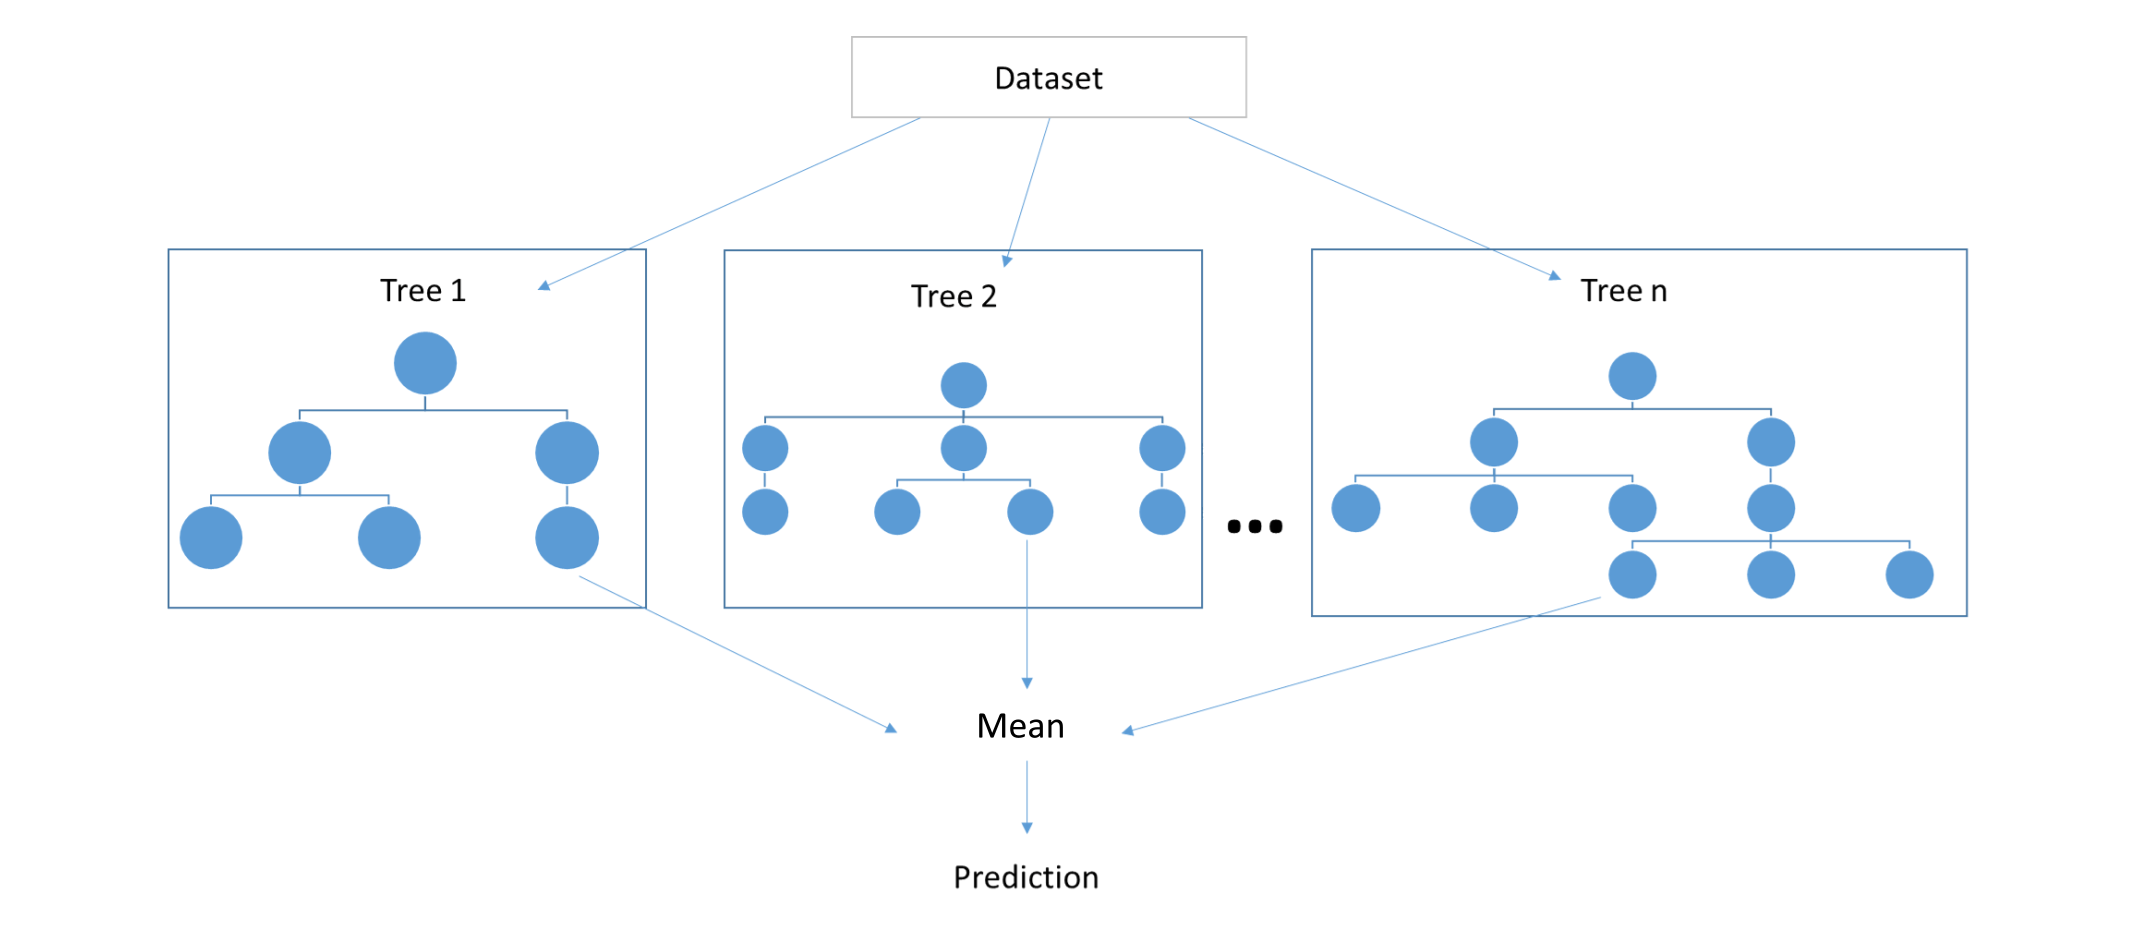
\includegraphics[scale=0.15]{graphs/RandomForest.png}
        \caption{Random Forest Regressor}
        \label{fig:N20}
    \end{figure}
\end{frame}
    
\begin{frame}
    \frametitle{Random Forest}
    More about Random Forest:
    \begin{itemize}
    \item Random Forest differs from bagging decision trees because each of the trees are trained from a subset of the features with a process known as the Random Subspace method. 
    \item Random Forest remedies a single decision tree's tendency to overfit the data and controls variance.
    \item Compared to Neural Networks, it can give good results with fewer data samples. 
    \item Low computational cost
    \end{itemize}
\end{frame}
\begin{frame}
    \frametitle{Random Forest}
    For our purposes, we used the Random Forest regressor from sklearn, which defaults to 100 trees and uses mean squared error as criterion to measure the quality of a split. (RMSE: 0.32)
    \begin{figure}[H]
        \centering
        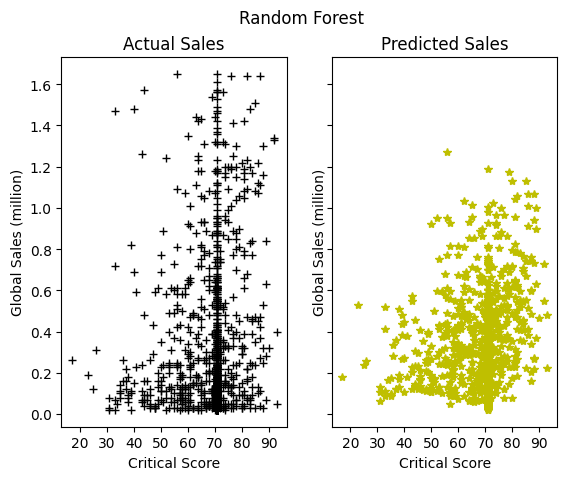
\includegraphics[scale=0.5]{graphs/random_forest.png}
        \caption{Random Forest Regressor}
        \label{fig:N20}
    \end{figure}
\end{frame}